\subsection{Relaxed shared CountMin sketch}
\label{ivl-ssec:countMin}

In this Section we present a relaxed CountMin sketch. Section~\ref{ivl-sssec:cm} presents a concurrent
IVL implementation, and shows that this implementation isn't linearizable.
Section~\ref{ivl-sssec:relaxed-cm} presents the $r$-relaxed IVL CM sketch.

\subsubsection{IVL CountMin sketch}
\label{ivl-sssec:cm}

Cormode et al. propose the \emph{CountMin (CM)} sketch~\cite{CountMin}, which
estimates the frequency of an item $a$, denoted $f_a$, in a data stream, where the data stream
is over some alphabet $\Sigma$. The CM sketch supports two operations: {\sc update}($a$),
which updates the object based on $a \in \Sigma$, and {\sc query}($a$), which returns
an estimate on the number of {\sc update}($a$) calls that preceded the query. \inred{The number
of {\sc update} operations that precede a query is called the \emph{stream length},
generally denoted by $N$.}

The sequential algorithm's underlying data structure is a matrix $c$ of $w \times d$ counters,
for some parameters $w,d$ determined according to the desired error and probability bounds.
The sketch uses $d$ hash functions $h_i: \Sigma \mapsto [1,w]$, for $1 \leq i \leq d$.
The hash functions are generated using the random coin flip vector $\vv{c}$,
and have certain mathematical properties whose details are not essential for understanding this paper.
The algorithm's input (i.e., the schedule) is generated by a so-called \emph{weak adversary}, namely,
the input is independent of the randomly drawn hash functions.
% These hash functions are drawn randomly by a
% \emph{weak adversary}, i.e., the schedule is independent from the hash functions.

The CountMin sketch, denoted $CM(\vv{c})$, is illustrated in Figure~\ref{ivl-img:cmSketch}, and its
pseudo-code is given in Algorithm~\ref{ivl-alg:count-min}.
On {\sc update}($a$), the sketch increments counters $c[i][h_i(a)]$ for every
$1 \leq i \leq d$. {\sc query}($a$) returns $\hat{f}_a=\min_{1 \leq i \leq d}\{c[i][h_i(a)]\}$.

\begin{algorithm}
    \begin{algorithmic}[1]
        % \begin{multicols}{2}

        \State array $c[1 \dots d][1 \dots w]$ \Comment{Initialized to $0$}
        \State hash functions $h_1, \dots h_d$ \Comment{$h_i: \Sigma \mapsto [1,w]$, initialized using $\vv{c}$}
        \Statex
        \Procedure{update}{$a$}
        \For{$i : 1 \leq i \leq d$}
        \State atomically increment $c[i][h_i(a)]$ \label{ivl-l:counter-inc}
        \EndFor
        \EndProcedure

        % \columnbreak

        \Procedure{query}{$a$}
        \State $min \gets \infty$
        \For{$i : 1 \leq i \leq d$}
        \State $c \gets c[i][h_i(a)]$ \label{ivl-l:read-min}
        \State \algorithmicif\ $min > c$ \ \algorithmicthen\ $min \gets c$ \label{ivl-l:min-update}
        \EndFor
        \State \textbf{return} $min$
        \EndProcedure
    % \end{multicols}
    \end{algorithmic}
    \caption{CountMin($\vec{c}$) sketch.}
    %\caption{CountMin($\vv{c}$) sketch.}
    \label{ivl-alg:count-min}
\end{algorithm}

Cormode et al. show that, for desired bounds $\delta$ and $\alpha$, given appropriate values of $w$ and $d$, with probability
at least $1-\delta$, the estimate of a query returning $\hat{f}_a$ is bounded by $f_a \leq \hat{f}_a \leq f_a + \alpha N$,
where \inred{$N$ is the number of elements in the stream} and $f_a$ is the ideal value.
Thus, for $\epsilon= \alpha N$, CM is a sequential $(\epsilon, \delta)$-bounded
object. Its sequential specification distribution is $\{CM(\vv{c})\}_{\vv{c} \in \Omega^\infty}$.

% \afterpage{
  \begin{figure}
    \begin{center}
     \includegraphics[width=0.4\textwidth,trim=10 0 30 10,clip]{graphics/ivl/cmSketch.png}
      \caption[The LOF caption]{An example CountMin sketch, of size $w \times d$, where $h_1(a)=6$, $h_2(a)=4$ and $h_d(a)=w$.\footnotemark}
     \label{ivl-img:cmSketch}
    \end{center}
  \end{figure}
  \footnotetext{Source: \url{https://stackoverflow.com/questions/6811351/explaining-the-count-sketch-algorithm}, with alterations.}
% }
% \begin{figure}[b]
%     \centering
%     \includegraphics[width=0.3\textwidth,trim=10 0 30 10,clip]{images/cmSketch.png}
%     %\caption{An example CountMin sketch, of size $w \times d$, where $h_1(a)=6$, $h_2(a)=4$ and $h_d(a)=w$.\footnote{Image from https://stackoverflow.com/questions/6811351/explaining-the-count-sketch-algorithm}}
%     \caption[Caption for LOF]{An example CountMin sketch, of size $w \times d$, where $h_1(a)=6$, $h_2(a)=4$ and $h_d(a)=w$.\protect\footnote{Image from https://stackoverflow.com/questions/6811351/explaining-the-count-sketch-algorithm}}
%     \label{ivl-img:cmSketch}
% \end{figure}

Proving an error bound for an efficient parallel implementation of the CM sketch is not trivial.
Any linearizable implementation, and even an $r$-relaxed linearizable, such as that of
Rinberg et al.~\cite{rinberg2019fast}, requires the query to take an
atomic snapshot of the matrix~\cite{ovens2019strongly}, which we forgo in Algorithm~\ref{ivl-alg:count-min}.
Distributional linearizability~\cite{alistarh2018distributionally} necessitates an analysis of the error bounds
directly in the concurrent setting, without leveraging the sketch's existing analysis for the sequential setting.

Instead, we utilize IVL to leverage the sequential analysis for a parallelization that
is not strongly linearizable (or indeed linearizable), without using a
snapshot. Consider the straightforward parallelization of the CM sketch,
whereby the operations of Algorithm~\ref{ivl-alg:count-min} may be invoked concurrently
and each counter is atomically incremented \inred{(e.g., using a FAA atomic operation~\cite{atomic-inc})} on
line~\ref{ivl-l:counter-inc} and read on line~\ref{ivl-l:read-min}. We call
this parallelization $PCM$. We next prove that it is IVL.% Its error analysis then follows from Theorem~\ref{ivl-thm:SIVL-bound}.


\begin{lemma}
    %The straightforward parallelization of the CM sketch Algorithm~\ref{ivl-alg:count-min} is IVL.
    $PCM$ is an IVL implementation of $CM$.
    \label{ivl-lmma:count-min-ivl}
\end{lemma}
\begin{proof}
    Let $H$ be a history of an execution $\sigma$ of $PCM$.
    Let $H_1$ be a linearization of $H^?$ such that every query is linearized prior to every
    concurrent update, and let $H_2$ be a linearization of $H^?$ such that every query is linearized after every
    concurrent update. Let $\sigma_i$ for $i=1,2$ be a sequential execution of $CM$ with history $H_i$.
    Consider some $Q=${\sc query}($a$) that returns in $H$, and let $U_1,\dots,U_k$ be the concurrent updates to $Q$.
    
    Denote by $c_\sigma(Q)[i]$ the value read by $Q$ from $c[i][h_i(a)]$ in line~\ref{ivl-l:read-min} of Algorithm~\ref{ivl-alg:count-min}
    in an execution $\sigma$.
    % Let $c_a = \left\{c[1][h_1(a)], \dots, c[d][h_d(a)]\right\}$ be the vector of counters associated with $a$ as seen by $Q$ in $H$.
    % In a similar fashion Let $c_a^i= \left\{c^i[1][h_1(a)], \dots, c^i[d][h_d(a)]\right\}$ be the vector
    % as seen by $Q$ in $H_i$.
    As processes only increment counters, for every $1 \leq i \leq d$, $c_{\sigma}(Q)[i]$ is at least
    $c_{\sigma_1}(Q)[i]$ (the value when the query starts) and at most $c_{\sigma_2}(Q)[i]$ (the value when
    all updates concurrent to the query complete). Therefore,
    $c_{\sigma_1}(Q)[i] \leq c_{\sigma}(Q)[i] \leq c_{\sigma_2}(Q)[i]$.

    Consider a randomly sampled coin flip vector $\vv{c} \in \Omega^\infty$.
    Let $j$ be the loop index the last time query $Q$ alters the value of its local variable $min$ (line~\ref{ivl-l:min-update}),
    i.e., the index of the minimum read value.
    As a query in a history of $CM(\vv{c})$ returns the minimum value in the array, $\text{ret}(Q, \tau_{CM(\vv{c})}(H_1)) \leq c_{\sigma_1}(Q)[j]$. Furthermore, $\text{ret}(Q, \tau_{CM(\vv{c})}(H_2))$
    is at least $c_{\sigma}(Q)[j]$, otherwise $Q$ would have read this value and returned it instead. Therefore:
    \[
        \text{ret}(Q, \tau_{CM(\vv{c}))}(H_1)) \leq \text{ret}(Q, H(PCM, \sigma, \vv{c})) \leq \text{ret}(Q, \tau_{CM(\vv{c})}(H_2))
    \]
    As needed.
\end{proof}

Combining Lemma~\ref{ivl-lmma:count-min-ivl} and Theorem~\ref{ivl-thm:SIVL-bound}, and by utilizing the sequential
error analysis from~\cite{CountMin}, we have shown the following corollary:
\begin{corollary}
    Consider a concurrent history $H$ of PCM with parameters $(\epsilon, \delta)$, with a stream of length $N$.
    Let $\hat{f}_a$ be a return value from query $Q$ with parameter $a$ in $H$. Let $f_a^\text{start}$ be the ideal frequency of element $a$
    \inred{at the invocation of $Q$}, and let $f_a^\text{end}$ be the ideal frequency of element $a$ \inred{at the response of $Q$}. Then:
    \[ f_a^\text{start} \leq \hat{f}_a \leq f_a^\text{end} + \epsilon \text{ with probability at least } 1-\delta.\]
\end{corollary}
\inred{
\begin{proof}
    Let $CM$ be a sequential $(\epsilon, \delta)$-bounded object. Lemma~\ref{ivl-lmma:count-min-ivl} proves that $PCM$
    is an IVL implementation of $CM$, therefore, by Theorem~\ref{ivl-thm:SIVL-bound}, PCM implements a concurrent
    $(\epsilon, \delta)$-bounded object.

    Consider some concurrent history $H$ containing $N$ update operations, and consider some query $Q$ of element $a$
    that returns in $H$. Let $H^{\text{start}}$ be the prefix of $H$ up to the invocation of $Q$, where all pending operations
    are removed. Let $f_a^\text{start}$ be the number of update operations in $H^{\text{start}}$ with parameter $a$. As each
    update operation increments the counters $Q$ reads, and they all precede $Q$, then $f_a^\text{start} \leq v^{\mathcal{I}}_{min}(H,Q)$.
    
    Let $H^{\text{end}}$ be the prefix of $H$ up to the response of $Q$, where all pending operations
    are completed.Let $f_a^\text{end}$ be the number of update operations in $H^{\text{end}}$ with parameter $a$. As each
    update operation increments the counters $Q$ reads, then $f_a^\text{end} \geq v^{\mathcal{I}}_{min}(H,Q)$.
    Therefore:
    \[ f_a^\text{start} - \epsilon \leq \hat{f}_a \leq f_a^\text{end} + \epsilon \text{ with probability at least } 1-\delta.\]

    This can be further improved by noting that the $Q$ returns at least $f_a^\text{start}$, as it cannot read the counters
    with values less than $f_a^\text{start}$. Therefore:
    \[ f_a^\text{start} \leq \hat{f}_a \leq f_a^\text{end} + \epsilon \text{ with probability at least } 1-\delta.\]
\end{proof}
}

The following example demonstrates that $PCM$ is not a linearizable implementation of $CM$.

\begin{example}
    Consider the following execution $\sigma$ of $PCM$: Assume that $\vv{c}$ is such that $h_1(a)=h_2(a)=1$, $h_1(b)=2$ and $h_2(b)=1$.
    Assume that initially
    \[ c=\CM{1}{4}{2}{3}. \]
    First, process $p$ invokes $U=${\sc update}$(a)$ which increments $c[1][1]$ to $2$ and stalls.
    Then, process $q$ invokes $Q_1=${\sc query}$(a)$ which reads $c[1][1]$ and $c[2][1]$ and returns $2$,
    followed by $Q_2=${\sc query}$(b)$ which reads $c[1][2]$ and $c[2][1]$ and returns $2$. Finally, process $p$ increments $c[2][1]$ to be $3$.

    Assume by contradiction that $H$ is a linearization of $\sigma$, and $H \in CM(\vv{c})$.
    The return values imply that $U \prec_H Q_1$ and $Q_2 \prec_H U$. As $H$ is a linearization, it maintains
    the partial order of operations in $\sigma$, therefore $Q_1 \prec_H Q_2$. A contradiction.
    % Consider a CM sketch of size $2 \times 2$, such that $h_1(a)=h_2(a)=1$ and $h_1(b)=2, h_2(b)=1$ for
    % two elements $a,b \in \Sigma$. Consider a \CM{1}{4}{2}{3}, and consider process $p$
    % which executes $Q_1=${\sc query}$(a)$ followed by $Q_1=${\sc query}$(b)$, and process
    % $q$ which executes {\sc update}$(a)$ concurrently to the queries. Let $H$ be the arising
    % history, and let $f$ be the mapping under linearizability. Query $Q_1$ may read
    % \CM{2}{4}{2}{3} thereby returning $2$, implying $U \prec_{f(H)} Q_1$.
    % $Q_2$ may read the same state thereby returning $2$, implying $Q_2 \prec_{f(H)} U$.
    % However, $Q_1 \prec_{f(H)} Q_2$ due to process order.
\end{example}


% \begin{example}
%     Consider a CM sketch of size $2 \times 2$, such that $h_1(a)=h_2(a)=1$ and $h_1(b)=2, h_2(b)=1$ for
%     two elements $a,b \in \Sigma$. Consider a \CM{1}{4}{2}{3}, and consider process $p$
%     which executes $Q_1=${\sc query}$(a)$ followed by $Q_1=${\sc query}$(b)$, and process
%     $q$ which executes {\sc update}$(a)$ concurrently to the queries. Let $H$ be the arising
%     history, and let $f$ be the mapping under linearizability. Query $Q_1$ may read
%     \CM{2}{4}{2}{3} thereby returning $2$, implying $U \prec_{f(H)} Q_1$.
%     $Q_2$ may read the same state thereby returning $2$, implying $Q_2 \prec_{f(H)} U$.
%     However, $Q_1 \prec_{f(H)} Q_2$ due to process order.
% \end{example}

% From Theorem~\ref{ivl-thm:SIVL-bound} we have parallelized the CM sketch while
% preserving bounds. The next step is to calculate these bounds. Note that
% the CountMin sketch is an $(\epsilon n, \delta)$-bounded object. Therefore,
% from Theorem~\ref{ivl-thm:SIVL-bound}, the concurrent implementation is also
% $(\epsilon n, \delta)$-bounded. More accurately, Cormode et al. show that if $f_a$ is the true count of $a$, and
% the stream length is $n$, then the approximation $\hat{f}_a$
% is in the range $f_a \leq \hat{f}_a \leq f_a + \epsilon n$, with
% probability at least $1-\delta$. In fact, the left inequality is true with
% probability $1$, it is only the right hand inequality which is bound with probability.
% Consider $k$ concurrent
% writes to some query $Q$ of count $a$, of which $l \leq k$ are {\sc update} operations
% which parameter $a$ (i.e., if the true value before is $f_a$,
% then true value after is $f_a + l$), then the returned value is in the
% range $f_a \leq \hat{f}_a \leq f_a + l + \epsilon(n + k)$
% with probability at least $1-\delta$.

\subsubsection{Relaxed IVL CM sketch}
\label{ivl-sssec:relaxed-cm}

Using the $r$-relaxed IVL form, we can create a buffered CM sketch
by using a similar framework to Rinberg et al.~\cite{rinberg2019fast}. The
\textsc{update} operations are buffered locally by updating threads until a certain threshold
is reached. The resulting matrix is then merged into the shared CM sketch,
which is updated element by element. 

This buffered approach allows for far better memory locality. Rather than every
\textsc{update} operating on shared memory, most operations are local. This
leads to better cache utilization, and forgoes expensive NUMA memory accesses.

In Rinberg et al., a \textsc{query} takes a strongly linearizable snapshot of the
current global state, and applies the query
to it.  In a CM sketch, a linearizable snapshot is an expensive operation -- it requires
an atomic snapshot. Using an IVL query
forgoes the need for a strongly linearizable snapshot, while retaining error bounds.

The buffered IVL CM sketch is $r$-relaxed IVL with respect to $\mathcal{H}_{CM}$, where
$r=2Wb$, where $W$ is the number of worker threads and $b$ is the local buffer size (i.e.,
the number of updates processed between propagations).

The error analysis follows from the relaxation and the definition of IVL. Consider some query $Q$ on $a$
that returns $v$, and let $S^{start}$ and $S^{end}$ be the state of the system at the start and end of
$Q$'s execution, respectively.
%Let $N$ be the length of the stream and $v^{start}$ be the number of times $a$ appears in the stream before $S^{start}$.
\inred{Let $v^{start}$ be the number of times $a$ appears in the stream before $S^{start}$, let
$v^{end}$ be the number of times $a$ appears in the stream before $S^{end}$, and let $N^{end}$
be the length of the stream at $S^{end}$.}
\[ v^{start} - r \leq v \leq  v^{end} + \epsilon N^{end}. \]